\scanpage{48}
% archive foliation: 47
% The printed sheet is upside down in the supplied scan; reading order below follows its text upright.
ACADEMIE DE MONTPELLIER

\texttt{----------}

JC/JV

LE RECTEUR DE L'ACADEMIE DE MONTPELLIER

Chancelier des Universités

VU\qquad la loi N° 68-978 du 12 novembre 1968
d'orientation de l'enseignement supérieur
et notamment son article 18

VU\qquad la démission présentée par M. le Profes-\\
seur Jacques ROUZAUD, administrateur
provisoire de l'Université de
MONTPELLIER II

A R R E T E

\texttt{-----------}

\uline{Article premier}.

La démission de M. le Professeur Jacques ROUZAUD
de ses fonctions d'administrateur provisoire de
l'Université de Montpellier II est acceptée à compter
du 26 juin 1978 et l'arrêté rectoral du 15 décembre
1977 est abrogé à la même date.

\uline{Article deux.}

Monsieur Yvan MEYERHOEFFER, Conseiller du Tribunal
Administratif de Montpellier, est chargé des fonctions
d'administrateur provisoire de l'Université de
Montpellier II à compter du 27 juin 1978 et jusqu'à
la date d'installation d'un président élu.

Fait à Montpellier, le 27 juin 1978

LE RECTEUR,

\figure{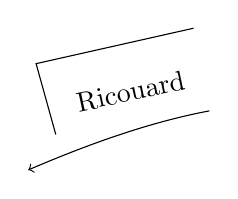
\begin{tikzpicture}[x=1cm,y=1cm]
\node[rotate=12] at (0,0) {\unsure{Ricouard}};
\draw (0.8,0.8)--(-1.2,0.35)--(-0.95,-0.55);
\draw[->] (1.0,-0.25) .. controls (0.2,-0.4) and (-0.6,-0.7) .. (-1.3,-1.0);
\end{tikzpicture}}

\uline{Diffusion} : liste D

n° 4027

MONTPELLIER, le 27 Juin 1978
